
\documentclass[xcolor={dvipsnames}]{beamer}
\usepackage{amsmath}
% \usepackage{beamerthemesplit} // Activate for custom appearance
\usepackage{hyperref}
\usepackage{ragged2e}
\usepackage{amssymb}
\usepackage{verbatim}
\usepackage{lmodern}
\usepackage{color}



\title{Recommender Systems}
\author{Schwartz}
\date{\today}



\begin{document}



\frame{\titlepage}

\frame
{
\frametitle{Recommender Systems: the ultimate win win?}

Stephen Covey's \emph{The 7 Habits of Highly Effective People} are:

\begin{enumerate}
\item[]  \textbf{Self-Mastery}
\item \emph{Be Proactive} in your Circle of Influence/Circle of Concern
\item \emph{Begin with the End in Mind}
\item \emph{Put First Things First}: 

\vspace{1em}
\begin{figure}

\begin{tabular}{|r||c|c|}
\hline
&Important& Not Important\\\hline\hline
Urgent & Do This & AVOID$^*$\\\hline
Not Urgent & Then this & Never do this\\\hline
\end{tabular}

\vspace{.5em}
$^*$Tyranny of the Urgent
\end{figure}

\vspace{.5em}

\item[]  \textbf{Interdependence}
\item \textcolor{red}{\underline{\emph{Think Win-Win}}: why are recommender systems win-wins?}
\item \emph{Seek First to Understand, Then to be Understood}
\item \emph{Synergize}
\item[]  \textbf{Sharpening the Saw}
\item \emph{"Always be Getting Better"}
\end{enumerate}

}


\frame
{
\frametitle{Objectives}

\huge
\begin{itemize}
\item Recommender Systems
\begin{itemize}
\item \textcolor{gray}{Popularity}
\item \textcolor{gray}{Content-Based}
\item \textbf{Collaborative Filtering} 
\end{itemize}
\item Cold Start\\
\vspace{.5em}
\item Matrix Factorization
\begin{itemize}
\item SVD vs UVD vs NMF
\item UVD via SGD
\item Bias modeling
\item Regularization
\item \textcolor{gray}{Performance}
\end{itemize}
\item Evalutation
\end{itemize}


}


\frame
{
\frametitle{The Ultimate Win-Win Opportunity}

\begin{itemize}
\item Know what the user will \emph{enjoy}: e.g., Facebook
\item Know what the user will \emph{click}: e.g., GoogleAds
\item Know what the user will \emph{buy}: e.g., Amazon
\end{itemize}

\onslide<2->{
\begin{figure}
\centering
\fbox{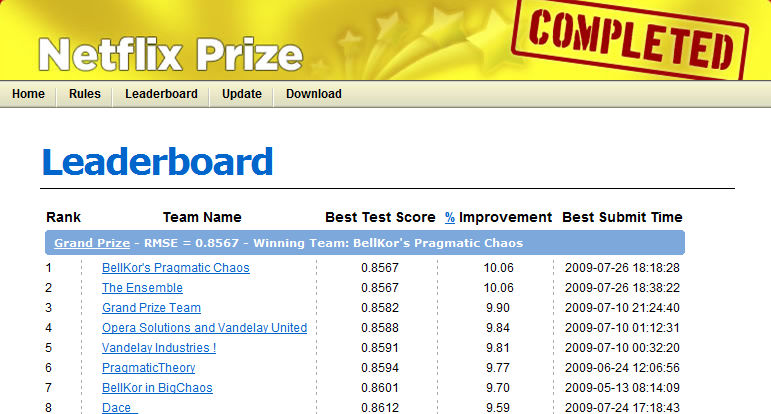
\includegraphics[width=3in]{stuff/NetflixPrize.png}}
\end{figure}}

\begin{itemize}
\tiny
\item[Train:]<2-> 480,189 users gave 17,770 movies 100,480,507 ratings (1-5)
\item[Test:]<2-> RMSE for 2,817,131 ratings; average user rated over 200 movies;
average movie rated by over 5000 users
\item<2-> Netflix would award the \$1M prize for beating Netflix's own model by 10\% 
(RMSE of 0.9514 to 0.8563)
\item<3-> It took almost 3 years; ``progress prizes'' were awarded every year; 8.43\%
improvement after one year
\item<3-> Final top two teams were merger of several top teams and Netflix never implemented 
the winning solution
\end{itemize}

}


\frame
{
\frametitle{Types of Recommender Systems}

\begin{columns}
\begin{column}{.5\textwidth}
\small

\onslide<2->{\textbf{Popularity}}

\begin{itemize}
\item<2-> Same recommendation for all
\item<2-> Based on item popularity
\item<2-> E.g. Twitter ``Moments"
\end{itemize}
${}$\\
\onslide<3->{\textbf{Content-Based}}
\begin{itemize}
\item<3-> I.e., Content Filtering
\item<3-> Predictions using item features 
\item[-]<3-> Does not utilize user behavior 
\item[-]<3-> Does utilize search criterion
\item<3-> E.g., Pandora Radio
\end{itemize}

\end{column}
\begin{column}{.5\textwidth}

\small

\color{Maroon}
\onslide<4->{\textbf{Collaborative Filtering}}

\begin{itemize}
\color{Maroon}
\item<4-> User-User similarity
\item<4-> Item-Item similarity
\item<4->[-] Does utilize user behavior 
\item<4->[-] Does not utilize item content
\item<4-> E.g., Netflix, Amazon
\end{itemize}
${}$\\

\color{NavyBlue}
\onslide<5->{\textbf{Matrix Factorization Methods}}
\begin{itemize}
\color{NavyBlue}
\item<5-> Find and Leverage 
\item<5->[] Latent Features (factors)
\item<5-> Expands NMF methodology
\end{itemize}

\end{column}
\end{columns}
${}$\\

\onslide<6->{\begin{figure}\textbf{Many Recommender Systems are Hybrids of These!}\end{figure}}

}

\frame
{
\begin{figure}
\Huge
Collaborative Filtering
\end{figure}

}


\frame
{
\frametitle{Utility Matrix (the data)}

$n$ users and $p$ items 

\begin{columns}
\begin{column}{.5\textwidth}

\begin{table}
\begin{tabular}{|l|ccccc|}
\hline
  & \multicolumn{5}{|c|}{Item} \\
    & A & B & C & D & $\cdots$ \\ \hline
Al & 1 & \textcolor{gray}{?} & 2 & \textcolor{gray}{?} &\\
Bob & \textcolor{gray}{?} & 2 & 3 & 4 &\\
Cat & 3 & \textcolor{gray}{?} & 1 & 5&\\
Dan & \textcolor{gray}{?} & 2 & \textcolor{gray}{?} & \textcolor{gray}{?}& \\
Ed & 2 &   \textcolor{gray}{?} & \textcolor{gray}{?} & 1&\\
$\vdots$ &&&&&\\ \hline
\end{tabular}
\caption{Netflix Rating Data}
User-Item Utility Matrix
\end{table}


\end{column}
\begin{column}{.5\textwidth}

\begin{table}
\begin{tabular}{|l|ccccc|}
\hline
  & \multicolumn{5}{|c|}{Item} \\
    & A & B & C & D & $\cdots$ \\ \hline
Al & 0 & \textcolor{gray}{?} & 0 & \textcolor{gray}{?} &\\
Bob & \textcolor{gray}{?} & 0 & 1 & 1 &\\
Cat & 1 & \textcolor{gray}{?} & 0 & 1&\\
Dan & \textcolor{gray}{?} & 0 & \textcolor{gray}{?} & \textcolor{gray}{?}& \\
Ed & 0 &   \textcolor{gray}{?} & \textcolor{gray}{?} & 0 &\\
$\vdots$ &&&&&\\ \hline
\end{tabular}
\caption{Youtube Next Data}
User-Item Utility Matrix
\end{table}


\end{column}
\end{columns}

\Huge
$$\textcolor{white}{O(n\times  n \times p)}$$

}



\frame
{
\frametitle{User Similarity}

$n$ users and $p$ items 

\begin{columns}
\begin{column}{.5\textwidth}

\begin{table}
\begin{tabular}{|l|ccccc|}
\hline
  & \multicolumn{5}{|c|}{Item} \\
    & A & B & C & D & $\cdots$ \\ \hline
\textcolor{red}{Al} & \textcolor{red}{1} & \textcolor{gray}{?} & \textcolor{red}{2 }& \textcolor{gray}{?} &\\ 
Bob & \textcolor{gray}{?} & 2 & 3 & 4 &\\ 
\textcolor{red}{Cat} & \textcolor{red}{3} & \textcolor{gray}{?} & \textcolor{red}{1} & \textcolor{red}{5}&\\ 
Dan & \textcolor{gray}{?} & 2 & \textcolor{gray}{?} & \textcolor{gray}{?}& \\
Ed & 2 &   \textcolor{gray}{?} & \textcolor{gray}{?} & 1&\\
$\vdots$ &&&&&\\ \hline
\end{tabular}
\caption{Netflix Rating Data}
User-Item Utility Matrix
\end{table}


\end{column}
\begin{column}{.5\textwidth}

\begin{table}
\begin{tabular}{|l|ccccc|}
\hline
  & \multicolumn{5}{|c|}{Item} \\
    & A & B & C & D & $\cdots$ \\ \hline
Al & 0 & \textcolor{gray}{?} & 0 & \textcolor{gray}{?} &\\
Bob & \textcolor{gray}{?} & 0 & 1 & 1 &\\
Cat & 1 & \textcolor{gray}{?} & 0 & 1&\\
Dan & \textcolor{gray}{?} & 0 & \textcolor{gray}{?} & \textcolor{gray}{?}& \\
Ed & 0 &   \textcolor{gray}{?} & \textcolor{gray}{?} & 0 &\\
$\vdots$ &&&&&\\ \hline
\end{tabular}
\caption{Youtube Next Data}
User-Item Utility Matrix
\end{table}


\end{column}
\end{columns}

\Huge
$$O(n\times  n \times p)$$

}




\frame
{
\frametitle{Item Similarity}

$n$ users and $p$ items 

\begin{columns}
\begin{column}{.5\textwidth}

\begin{table}
\begin{tabular}{|l|ccccc|}
\hline
  & \multicolumn{5}{|c|}{Item} \\
    & \textcolor{red}{A} & B & \textcolor{red}{C} & D & $\cdots$ \\ \hline
Al & \textcolor{red}{1} & \textcolor{gray}{?} & \textcolor{red}{2} & \textcolor{gray}{?} &\\
Bob & \textcolor{gray}{?} & 2 & \textcolor{red}{3} & 4 &\\
Cat & \textcolor{red}{3} & \textcolor{gray}{?} & \textcolor{red}{1} & 5&\\
Dan & \textcolor{gray}{?} & 2 & \textcolor{gray}{?} & \textcolor{gray}{?}& \\
Ed & \textcolor{red}{2} &   \textcolor{gray}{?} & \textcolor{gray}{?} & 1&\\
$\vdots$ &&&&&\\ \hline
\end{tabular}
\caption{Netflix Rating Data}
User-Item Utility Matrix
\end{table}


\end{column}
\begin{column}{.5\textwidth}

\begin{table}
\begin{tabular}{|l|ccccc|}
\hline
  & \multicolumn{5}{|c|}{Item} \\
    & A & B & C & D & $\cdots$ \\ \hline
Al & 0 & \textcolor{gray}{?} & 0 & \textcolor{gray}{?} &\\
Bob & \textcolor{gray}{?} & 0 & 1 & 1 &\\
Cat & 1 & \textcolor{gray}{?} & 0 & 1&\\
Dan & \textcolor{gray}{?} & 0 & \textcolor{gray}{?} & \textcolor{gray}{?}& \\
Ed & 0 &   \textcolor{gray}{?} & \textcolor{gray}{?} & 0 &\\
$\vdots$ &&&&&\\ \hline
\end{tabular}
\caption{Youtube Next Data}
User-Item Utility Matrix
\end{table}


\end{column}
\end{columns}

\Huge
$$O(p\times  p \times n)$$

}


\frame
{
\frametitle{What's easier: Item-Item Similarity or User-User Similarity?}



\begin{columns}

\hspace*{-1em}\begin{column}{.73\textwidth}
\vspace{-.5em}

\Large
\onslide<2->{\textbf{Item-Item}}

\begin{enumerate}
\item[]<3-> Many businesses have $n > p$
\item[]
\item<4-> Computation: $O(p\times  p \times n) < O(n\times  n \times p)$
\item<5-> Stability:\\ \emph{Item$_{\color{gray}a}$-Item$_{\color{gray}b}$}$>$\emph{User$_{\color{gray}1}$-User$_{\color{gray}2}$} overlap
\item<5->[]
\item<5->[] Less ``cold start'':\\ quicker to onboard new items 
\end{enumerate}

\end{column}
\begin{column}{.3\textwidth}

\onslide<3->{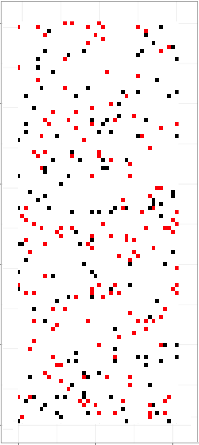
\includegraphics[width=1.35in]{stuff/overlap.png}}
\end{column}
\end{columns}
}


\frame
{
\frametitle{Similarity Metrics I}


\begin{itemize}
\item<2-> \textbf{Euclidean}
\begin{align*} 
Dist(a, b) = ||a-b||  = {}& \sqrt{\sum_i (a_i - b_i)^2}
\end{align*} 
\item<3-> \textbf{Pearson Correlation}
\begin{align*} 
Pearson(a, b) ={}& \frac{Cov(a, b)}{Std(a)Std(b)} = \frac{{\sum_i (a_i - \bar a)(b_i - \bar b)}}{\sqrt{\sum_i (a_i - \bar a)^2} \sqrt{\sum_i (b_i - \bar b)^2}}
\end{align*} 

\item<4-> \textbf{Cosine Similarity}
\begin{align*} 
Cos(\theta_{a, b}) ={}& \frac{a\cdot b}{||a|| ||b||} = \frac{{\sum_i a_i b_i }}{\sqrt{\sum_i a_i^2} \sqrt{\sum_i b_i^2}}
\end{align*} 
\item[] 
\item<5-> \emph{How do these work? \onslide<6->{\small What do they do for similarly rated items?}}

\end{itemize}



\vspace{2.5em}

}



\frame
{
\frametitle{Similarity Metrics II (similar $\rightarrow$ 1; dissimilar $\rightarrow$ 0)}


\begin{itemize}
\item \textbf{Euclidean}
\begin{align*} 
EuclideanSimilarity(a, b) ={}& \frac{1}{1+Dist(a, b)}
\end{align*} 
\item \textbf{Pearson Correlation}
\begin{align*} 
PearsonSimilarity(a, b) ={}& \frac{1}{2}+ \frac{1}{2} Pearson(a, b)
\end{align*} 

\item \textbf{Cosine Similarity}
\begin{align*} 
CosineSimilarity(a, b) ={}& \frac{1}{2}+ \frac{1}{2} Cos(\theta_{a, b})
\end{align*} 
\item<2-> \textbf{Jaccard Index}
\begin{align*}
JaccardSimilarity(a, b) ={}& \frac{|U_a \cap U_b|}{|U_a \cup U_b|}  
\end{align*} 
$\text{where }  U_{\text{item}} \text{ is the set of users who rated \emph{item}}$
\end{itemize}

}



\frame
{
\frametitle{Similarity Matrix and... {{how to make recommendation?}}}


\begin{columns}
\begin{column}{.5\textwidth}


\begin{table}
\begin{tabular}{|l|ccccc|}
\hline
  & \multicolumn{5}{|c|}{Item} \\
    & \textcolor{black}{a} & b & \textcolor{black}{c} & d & $\cdots$ \\ \hline
Al & \textcolor{black}{1} & \textcolor{gray}{?} & \textcolor{black}{2} & \textcolor{gray}{?} &\\
Bob & \textcolor{gray}{?} & 2 & \textcolor{black}{3} & 4 &\\
Cat & \textcolor{black}{3} & \textcolor{gray}{?} & \textcolor{black}{1} & 5&\\
Dan & \textcolor{gray}{?} & 2 & \textcolor{gray}{?} & \textcolor{gray}{?}& \\
Ed & \textcolor{black}{2} &   \textcolor{gray}{?} & \textcolor{gray}{?} & 1&\\
$\vdots$ &&&&&\\ \hline
\end{tabular}
\caption{Netflix Rating Data $X$}
\end{table}


\end{column}
\begin{column}{.5\textwidth}

\vspace{-.4em}
${}$\\${}$\\

\onslide<0>{
\begin{table}
\begin{tabular}{c||c|c|c|c||}
  & \multicolumn{4}{|c||}{Item}  \\
& a &  b &  c & $\cdots$ \\\hline \hline
item a &\textcolor{gray}{1}&$s_{12}$&$s_{13}$& \\ \hline
item b &\textcolor{gray}{$s_{21}$}&\textcolor{gray}{1}&$s_{23}$& \\ \hline
item c &\textcolor{gray}{$s_{31}$}&\textcolor{gray}{$s_{32}$}&\textcolor{gray}{1}& \\ \hline
$\vdots$ &&&& \\ \hline \hline
\end{tabular}
\caption{Similarity Matrix $S$}  
\end{table}
}
\end{column}
\end{columns}

\onslide<0>{
For user $u$ and item $i$ we can predict
user rating based on a weighted average of the other items the user has rated $I_{u}$ 
\Large
\begin{align*} 
PredictedRating(u, i) = {}& \frac{\sum_{j^* \in I_u} similarity(i,j^*) X_{i,j^*}}{\sum_{j^* \in I_u} similarity(i, j^*) }
\end{align*} 
}

}


\frame
{
\frametitle{Similarity Matrix and... {{how to make recommendation?}}}


\begin{columns}
\begin{column}{.5\textwidth}


\begin{table}
\begin{tabular}{|l|ccccc|}
\hline
  & \multicolumn{5}{|c|}{Item} \\
    & \textcolor{red}{a} & b & \textcolor{red}{c} & d & $\cdots$ \\ \hline
Al & \textcolor{red}{1} & \textcolor{gray}{?} & \textcolor{red}{2} & \textcolor{gray}{?} &\\
Bob & \textcolor{gray}{?} & 2 & \textcolor{red}{3} & 4 &\\
Cat & \textcolor{red}{3} & \textcolor{gray}{?} & \textcolor{red}{1} & 5&\\
Dan & \textcolor{gray}{?} & 2 & \textcolor{gray}{?} & \textcolor{gray}{?}& \\
Ed & \textcolor{red}{2} &   \textcolor{gray}{?} & \textcolor{gray}{?} & 1&\\
$\vdots$ &&&&&\\ \hline
\end{tabular}
\caption{Netflix Rating Data $X$}
\end{table}


\end{column}
\begin{column}{.5\textwidth}

\vspace{-.4em}
${}$\\${}$\\

\begin{table}
\begin{tabular}{c||c|c|c|c||}
  & \multicolumn{4}{|c||}{Item}  \\
& a &  b &  c & $\cdots$ \\\hline \hline
item a &\textcolor{gray}{1}&$s_{12}$&$s_{13}$& \\ \hline
item b &\textcolor{gray}{$s_{21}$}&\textcolor{gray}{1}&$s_{23}$& \\ \hline
item c &\textcolor{gray}{$s_{31}$}&\textcolor{gray}{$s_{32}$}&\textcolor{gray}{1}& \\ \hline
$\vdots$ &&&& \\ \hline \hline
\end{tabular}
\caption{Similarity Matrix $S$}  
\end{table}

\end{column}
\end{columns}

\onslide<0>{
For user $u$ and item $i$ we can predict
user rating based on a weighted average of the other items the user has rated $I_{u}$ 
\Large
\begin{align*} 
PredictedRating(u, i) = {}& \frac{\sum_{j^* \in I_u} similarity(i,j^*) X_{i,j^*}}{\sum_{j^* \in I_u} similarity(i, j^*) }
\end{align*} 
}

}



\frame
{
\frametitle{Similarity Matrix and... {{how to make recommendation?}}}


\begin{columns}
\begin{column}{.5\textwidth}

\begin{table}
\begin{tabular}{|l|ccccc|}
\hline
  & \multicolumn{5}{|c|}{Item} \\
    & a & b & c & d & $\cdots$ \\ \hline
\textcolor{black}{Al} & \textcolor{black}{1} & \textcolor{gray}{?} & \textcolor{black}{2 }& \textcolor{gray}{?} &\\ 
Bob & \textcolor{gray}{?} & 2 & 3 & 4 &\\ 
\textcolor{red}{Cat} & \textcolor{red}{3} & \textcolor{blue}{?} & \textcolor{red}{1} & \textcolor{red}{5}&\\ 
Dan & \textcolor{gray}{?} & 2 & \textcolor{gray}{?} & \textcolor{gray}{?}& \\
Ed & 2 &   \textcolor{gray}{?} & \textcolor{gray}{?} & 1&\\
$\vdots$ &&&&&\\ \hline
\end{tabular}
\caption{Netflix Rating Data $X$}
\end{table}


\end{column}
\begin{column}{.5\textwidth}

\vspace{-.4em}
${}$\\${}$\\

\begin{table}
\begin{tabular}{c||c|c|c|c||}
  & \multicolumn{4}{|c||}{Item}  \\
& a &  b &  c & $\cdots$ \\\hline \hline
item a &\textcolor{gray}{1}&$s_{12}$&$s_{13}$& \\ \hline
item b &\textcolor{gray}{$s_{21}$}&\textcolor{gray}{1}&$s_{23}$& \\ \hline
item c &\textcolor{gray}{$s_{31}$}&\textcolor{gray}{$s_{32}$}&\textcolor{gray}{1}& \\ \hline
$\vdots$ &&&& \\ \hline \hline
\end{tabular}
\caption{Similarity Matrix $S$}  
\end{table}

\end{column}
\end{columns}

\onslide<2->{
For user $u$ and item $i$ we can predict
user rating based on a weighted average of the other items the user has rated $I_{u}$ 
\Large
\begin{align*} 
PredictedRating(u, i) = {}& \frac{\sum_{j^* \in I_u} similarity(i,j^*) X_{i,j^*}}{\sum_{j^* \in I_u} similarity(i, j^*) }
\end{align*} 
}

}


\frame
{
\frametitle{Similarity Matrix and... {{how to make recommendation?}}}


\begin{columns}
\begin{column}{.5\textwidth}

\begin{table}
\begin{tabular}{|l|ccccc|}
\hline
  & \multicolumn{5}{|c|}{Item} \\
    & a & b & c & d & $\cdots$ \\ \hline
\textcolor{black}{Al} & \textcolor{black}{1} & \textcolor{gray}{?} & \textcolor{black}{2 }& \textcolor{gray}{?} &\\ 
Bob & \textcolor{gray}{?} & 2 & 3 & 4 &\\ 
\textcolor{red}{Cat} & \textcolor{red}{3} & \textcolor{blue}{?} & \textcolor{red}{1} & \textcolor{red}{5}&\\ 
Dan & \textcolor{gray}{?} & 2 & \textcolor{gray}{?} & \textcolor{gray}{?}& \\
Ed & 2 &   \textcolor{gray}{?} & \textcolor{gray}{?} & 1&\\
$\vdots$ &&&&&\\ \hline
\end{tabular}
\caption{Netflix Rating Data $X$}
\end{table}


\end{column}
\begin{column}{.5\textwidth}

\vspace{-.4em}
${}$\\${}$\\

\begin{table}
\begin{tabular}{c||c|c|c|c||}
  & \multicolumn{4}{|c||}{Item}  \\
& a &  b &  c & $\cdots$ \\\hline \hline
item a &\textcolor{gray}{1}&$s_{12}$&$s_{13}$& \\ \hline
item b &\textcolor{gray}{$s_{21}$}&\textcolor{gray}{1}&$s_{23}$& \\ \hline
item c &\textcolor{gray}{$s_{31}$}&\textcolor{gray}{$s_{32}$}&\textcolor{gray}{1}& \\ \hline
$\vdots$ &&&& \\ \hline \hline
\end{tabular}
\caption{Similarity Matrix $S$}  
\end{table}

\end{column}
\end{columns}

\onslide<1->{
For user $u$ and item $i$ we can predict
user rating based on a weighted average of the other items the user has rated $I_{u}$ 
\Large
\begin{align*} 
PredictedRating(u, i) = {}& \frac{\sum_{j^* \in I_u \color{blue}\cap N_i} similarity(i,j^*) X_{i,j^*}}{\sum_{j^* \in I_u \color{blue} \cap N_i} similarity(i, j^*) }
\end{align*} 
\footnotesize
$N_i$ is the set of the $n$ items most similar to item $i$
}



}



\frame
{
\frametitle{The Cold-Start Problem}



\begin{columns}
\begin{column}{.5\textwidth}



\underline{What about a new \emph{user}?}

\begin{itemize}
\item<2-> Why can't we give\\ this user recommendations?
\item[]
\item<3-> Ask user to rate \\5 item  on sign-up?
\item<4-> Popularity Recommender?
\end{itemize}



\end{column}
\begin{column}{.5\textwidth}


\onslide<5->{\underline{What about a new \emph{item}?}}

\begin{itemize}
\item<5-> Why can't we \\ recommend this item?
\item[]
\item<6-> ``New Content'' section? 
\item<7-> Content-Based? 
\item<7-> \textcolor{gray}{Popularity Recommender?}
\end{itemize}

\end{column}
\end{columns}



}


\frame
{
\Huge

\begin{figure}
Matrix Factorization Methods
\end{figure}
}

\frame
{
\frametitle{UV Decomposition (UVD)}

\color{Maroon}
\vspace{-3em}
\LARGE
\begin{align*} 
\underset{n\times p}{X} \approx{}& \underset{n\times \textcolor{red}{k}}{U}\;\;\underset{\textcolor{red}{k}\times p}{V}\\
X_{ij} \approx{}& U_{i \cdot}V_{\cdot j} = \hat X_{ij}
\end{align*}
$$\underset{U,V}{argmin} \sum_{i,j} (X_{ij} - {U_{i\cdot}}{V_{\cdot j}})^2$$

\vspace{.5em}
\normalsize 

\color{Black}

\begin{columns}
\hspace*{1em}
\begin{column}{.5\textwidth}
\LARGE
\onslide<2->{\textbf{SVD}}
\normalsize 
\begin{itemize}
\item<3-> \textcolor{NavyBlue}{$X = U\Sigma V^T$}
\item<4-> $U, V^T$ orthogonal 
\item<5-> single solution
\item<6-> analytical solution
\item<7->  \textcolor{NavyBlue}{no missing values}
\item<8->  \textcolor{Maroon}{singular values}
\end{itemize}
\end{column}
\hspace*{-5em}
\begin{column}{.5\textwidth}
\LARGE
\onslide<2->{\textbf{NMF}}
\normalsize 
\begin{itemize}
\item<3-> \textcolor{NavyBlue}{$X \approx WH; W, H \geq 0$}
\item<4-> $W, H$ non orthogonal 
\item<5-> non-unique solutions
\item<6-> iterative optimization
\item<7->  \textcolor{NavyBlue}{missing values okay}
\item<8-> \textcolor{Maroon}{tunable \textcolor{red}{$k$}}
\end{itemize}
\end{column}
\hspace*{-3em}\begin{column}{.5\textwidth}
\LARGE
\textbf{UVD}
\normalsize 
\begin{itemize}
\item<3-> \textcolor{NavyBlue}{$X \approx UV$}
\item<4-> $U, V$ non orthogonal 
\item<5-> non-unique solutions
\item<6-> iterative optimization
\item<7->  \textcolor{NavyBlue}{missing values okay}
\item<8-> \textcolor{Maroon}{tunable \textcolor{red}{$k$}}
\end{itemize}
\end{column}
\end{columns}

}




\frame
{
\frametitle{How do we learn $U$ and $V$?}

\begin{itemize}
\item<2-> \textbf{Gradient Descent} 
\vspace{-.5em}
\scriptsize

\begin{align*} 
\frac{\partial}{\partial U_{i'k}} \sum_{i,j} (X_{ij} - {U_{i\cdot}}\;\; {V_{\cdot j}})^2 = {}&  \sum_{j} -2(X_{i'j} - U_{i'k}\;\; V_{kj})V_{kj} \\
\frac{\partial}{\partial V_{kj'}} \sum_{i,j} (X_{ij} - {U_{i\cdot}}\;\; {V_{\cdot j}})^2 ={}& \sum_{i} -2(U_{ij'} - U_{ik}\;\; V_{kj'})U_{ik}
\end{align*}

\normalsize 

\item<3-> \textbf{Alternating Lease Squares (ALS)}
\begin{enumerate}

\footnotesize

\item Update $V_{\cdot j}$ using OLS: $X_{\cdot j} = \mathbf{U} {V_{\cdot j}} + \epsilon_{\cdot j}$

\tiny

$$\left[\begin{array}{cccc} & | && \\& | &&  \\& | &&  \end{array} \right] = \left[\begin{array}{c} \longrightarrow\longrightarrow \\ \longrightarrow\longrightarrow \\ \longrightarrow\longrightarrow  \end{array} \right] \left[\begin{array}{cccc} & \downarrow && \\&  \downarrow  && \\&  \downarrow  &&  \end{array} \right] $$

\footnotesize


\item Update $W_{i \cdot}$ using OLS: $X_{i\cdot}^T = \mathbf{V^T} {U_{i \cdot}^T}  + \epsilon_{i \cdot}^T$

\tiny
$$\arraycolsep=3pt%\def\arraystretch{2.2}
\left[\begin{array}{cccc} & \text{---} &\text{---}& \\&  && \\&  &&  \end{array} \right]^T = \left( \left[\begin{array}{c}\longrightarrow \longrightarrow \\ \\ \\ \end{array} \right] \left[\begin{array}{cccc} \downarrow & \downarrow & \downarrow& \downarrow \\ \downarrow&  \downarrow  & \downarrow& \downarrow  \\ \downarrow&  \downarrow  & \downarrow& \downarrow \end{array} \right] \right)^T$$
\end{enumerate}

\vspace{.5em}

\item<4->  \textbf{Lee and Seung's ``multiplicative update rules''}

\footnotesize 

Initialize non-negative $H$ and $W$; update with non-negativity constraint:
\begin{align*} 
W_{ik}' =  W_{ik} \frac{(X H^T)_{ik}}{(WHH^T)_{ik}} {}& \quad\quad H_{kj}' =  H_{kj} \frac{(W^T X)_{kj}}{(W^TWH)_{kj}}  \quad\quad  \quad\quad 
\end{align*} 

\end{itemize}

}







\frame
{
\frametitle{Numerical Estimation Comparisons}


\begin{columns}
\begin{column}{.5\textwidth}


\LARGE
\textbf{Alternating\\ Least Squares}
\normalsize 

\begin{itemize}
\item<2-> Simple idea/implementation
\item<2-> Parallelizes very well
\item<2-> Available in Spark/MLlib
\item<4-> \textcolor{Maroon}{Can handle NA's with care}
\end{itemize}



\LARGE
\textbf{Stochastic\\Gradient Decent}
\normalsize 

\begin{itemize}
\item<2-> Faster than ALS (per CPU) 
\item<3-> \textcolor{NavyBlue}{Need to turn learning rate}
\item<3-> \textcolor{NavyBlue}{Thought to outperform ALS}
\item<4-> \textcolor{Maroon}{Works with NA's}
\end{itemize}


\end{column}
\begin{column}{.5\textwidth}

\LARGE
\textbf{Multiplicative\\ Updates}
\normalsize 

\begin{itemize}
\item<2-> Easy implementation
\item<2-> Faster than SGD
\item<3-> \textcolor{NavyBlue}{No turning parameter}
\item<4-> \textcolor{Maroon}{Only works for NMF}
\item<4-> \textcolor{Maroon}{Can't handle NA's}
\end{itemize}


\end{column}
\end{columns}

}

\frame
{
\frametitle{UVD + SGD is best in class}

Used by the winning Netflix Challenge entry

\begin{itemize}
\item No need to impute missing values
\item Can model time dynamics (evolving user preference) 
\item Plus it can do all of these: 
\end{itemize}
\vspace{-1em}

\LARGE
$$\underset{U,V\only<2->{, \textcolor{NavyBlue}{\beta_{Ui}, \beta_{Ij}, \mu}}}{argmin}$$ 
$$\sum_{i,j} (X_{ij} -   \left(\only<2->{\textcolor{NavyBlue}{\mu + \beta_{Ui} + \beta_{Ij} +}} U_{i\cdot}V_{\cdot j})\right)^2$$ 
\onslide<4->{$$\textcolor{red}{+\; \lambda_1 \left(   ||U_{i\cdot}||^2 + ||V_{\cdot j}||^2  \right)}} \onslide<3->{\textcolor{Maroon}{+
\lambda_2 \left(    \beta_{Ui}^2 + \beta_{Ij}^2  \right)}} $$

\color{green}
\vspace{-1em}
\begin{figure}
\centering
\onslide<5->{\underline{\textbf{And Don't Forget $\boldsymbol k$!!!}}}
\end{figure}
}



\frame
{
\frametitle{Matrix Factorization Methods on the Netflix Challenge}

\begin{figure}
Netflix's in-house model achieves RMSE=0.9514

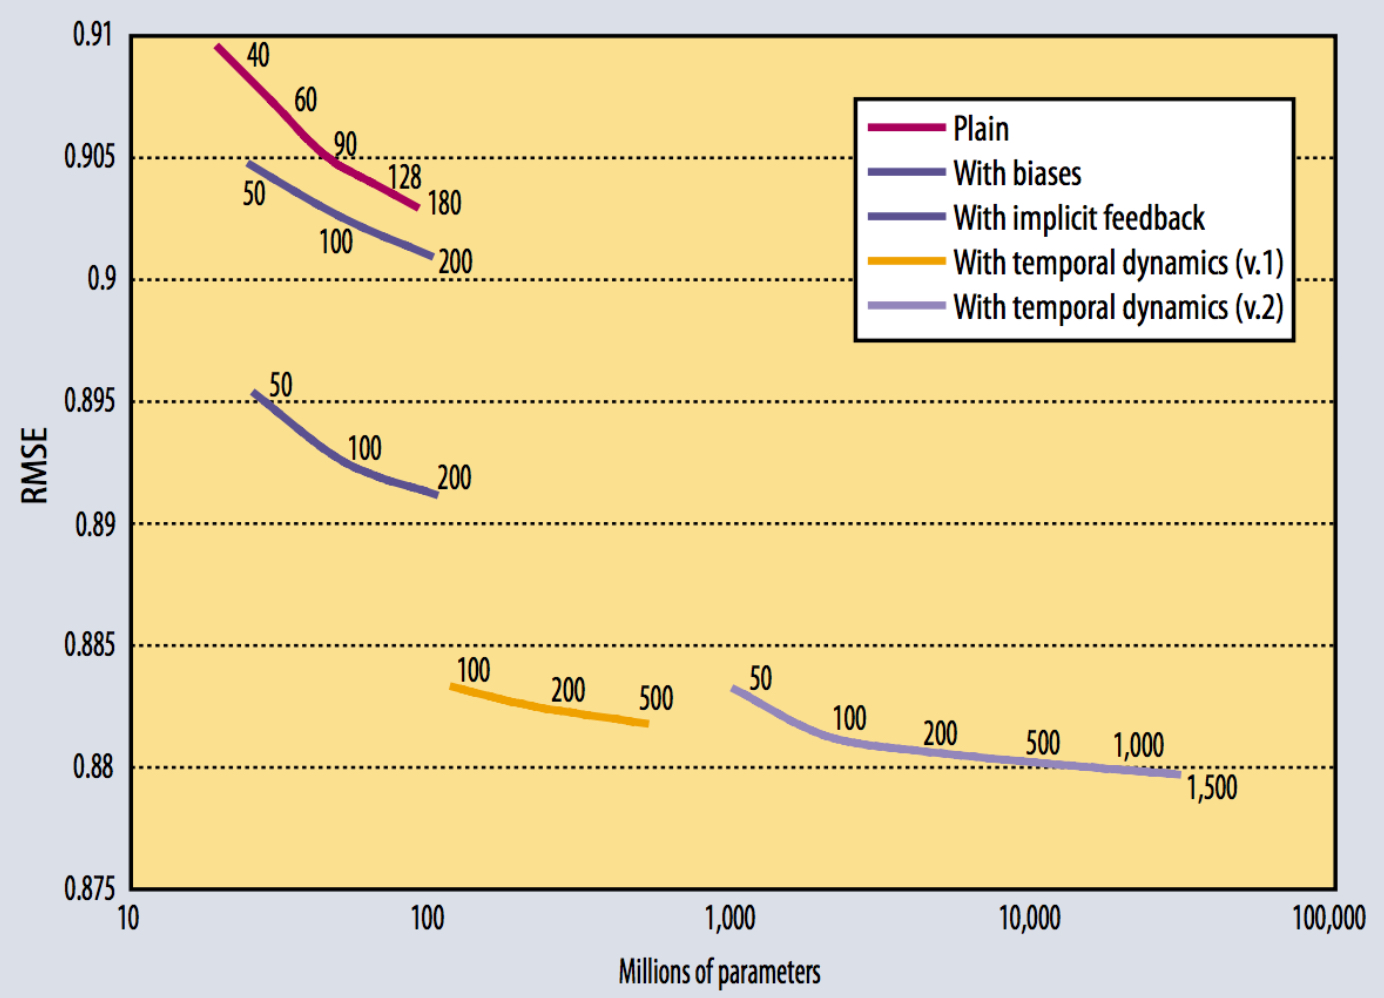
\includegraphics[width=3.75in]{stuff/RS_examples.jpg}

``Matrix Factorization Techniques for Recommender Systems"

\end{figure}

}


\frame
{
\frametitle{What are the \emph{``latent factors''}?}

\vspace{-2em}

\Huge
$$ \;\;X \quad = \; U \quad\;\; V\;\;$$ 

\normalsize
$$
\;\;\;\left[
\begin{array}{ccccccc}
&&&&&&\\
&&&&&&\\
&\textcolor{green}{*}&&&&&\\
&&&&&&\\
&&&&&&\\
&&&&&&\\
&&&&&&\\
&&&&&&\\
&&&&&&\\
\end{array}
\right] = 
\overset{\text{latents}}{
\left[
\begin{array}{c}
\\
\\
\textcolor{red}{\longrightarrow} \\
\\
\\
\\
\\
\\
\\
\end{array}
\right]}  
\left[
\begin{array}{ccccccc}
&\textcolor{blue}{\Big\downarrow}&&&&&\\
\end{array}
\right]\rotatebox{270}{\hspace{-1.6em} \scriptsize latents}
$$

\vspace{.5em}
\begin{itemize}
\item[] \hspace{.85in}\onslide<2->{\tiny \emph{so rows are ``item topics'' $\longrightarrow$}}\textcolor{blue}{\normalsize\emph{``item composition''}}
\item[] \normalsize\hspace{1.55in}\textcolor{red}{\emph{``user parts''}} \tiny \onslide<2->{\emph{$\longleftarrow$ and columns are ``user archetypes'' }} 
\end{itemize}

}


\frame
{
\frametitle{Wrap Up}

\color{NavyBlue}
\scriptsize
$$\underset{U,V\only<1->{, \textcolor{NavyBlue}{\beta_{Ui}, \beta_{Ij}, \mu}}}{argmin} 
\sum_{i,j} (X_{ij} -   \left(\only<1->{\textcolor{NavyBlue}{\mu + \beta_{Ui} + \beta_{Ij} +}} U_{i\cdot}V_{\cdot j})\right)^2  
\onslide<1->{\textcolor{NavyBlue}{+\; \lambda_1 \left(   ||U_{i\cdot}||^2 + ||V_{\cdot j}||^2  \right)}} \onslide<1->{\textcolor{NavyBlue}{+
\lambda_2 \left(    \beta_{Ui}^2 + \beta_{Ij}^2  \right)}} $$

\normalsize
\color{black}

\begin{columns}
\begin{column}{.55\textwidth}
\textbf{PROS}
\begin{itemize}
\item<2-> Regularization handles sparsity  
\item<3-> Fast dot product prediction
\item<4-> Latent feature interpretation
\item<5-> Can include auxiliary data
\item[]
\end{itemize}
\end{column}
\begin{column}{.55\textwidth}
\textbf{CONS}
\begin{itemize}
\item<6-> Re-factorizing new data is slow
\item<7-> No strong libraries available...
\item<8-> \textcolor{Maroon}{Fails at cold-start problem}
\item<9-> \textcolor{red}{Success is hard to nail down and thus hard to tune against} 
\end{itemize}

\end{column}
\end{columns}


${}$\\

\onslide<10->{
\underline{\textcolor{NavyBlue}{If you have a system it's easy to deploy:}}

\vspace{-.2em}
\begin{columns}
\begin{column}{.25\textwidth}
${}$
\end{column}
\begin{column}{.8\textwidth}

\begin{itemize}
\item[At Request Time:] Serve up best prediction score 
\item[or] use factorization dot product to prediction score 

\item<11->[During Down Time:] Compute pairwise similarity, $N_i$, and predictions
\item<11->[or] re-factorize matrix based on newly acquired data  

\end{itemize}

\end{column}
\end{columns}
}
}



\frame
{
\frametitle{BIG FINISH: \emph{Evaluating the Recommender}}


\underline{\textcolor{gray}{The difficulty is how do you get a system in the first place?}}

\begin{columns}

\hspace*{-1em}\begin{column}{.75\textwidth}

\only<1-1>{\begin{figure}\centering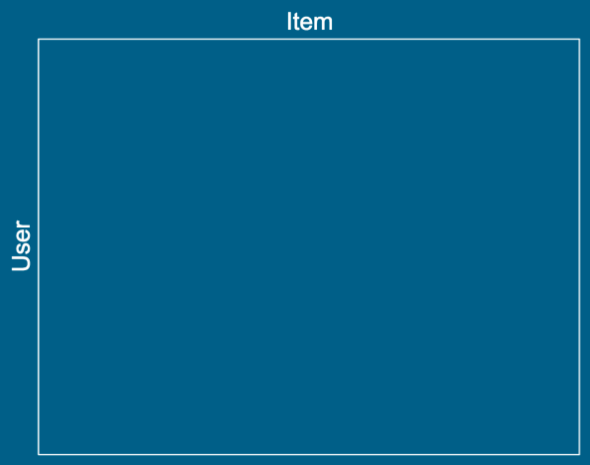
\includegraphics[width=2.5in]{stuff/rec2.png}\end{figure}}
\only<2-2>{\begin{figure}\centering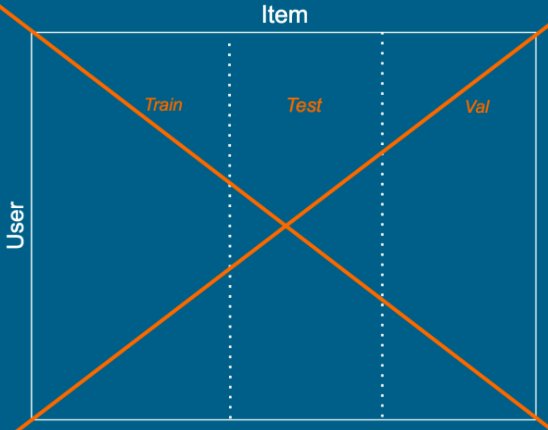
\includegraphics[width=2.5in]{stuff/rec1.png}\end{figure}}
\only<3-3>{\begin{figure}\centering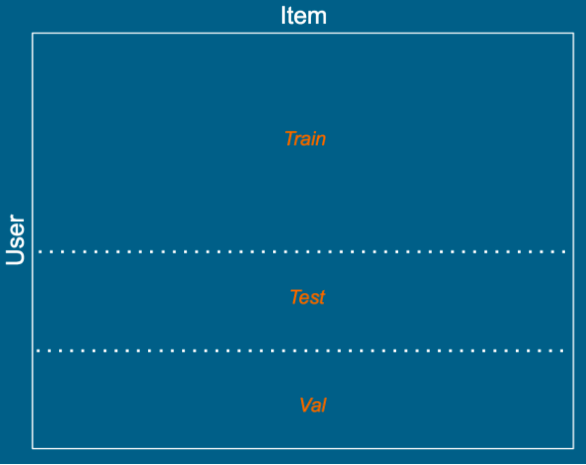
\includegraphics[width=2.5in]{stuff/rec4.png}\end{figure}}
\only<4-4>{\begin{figure}\centering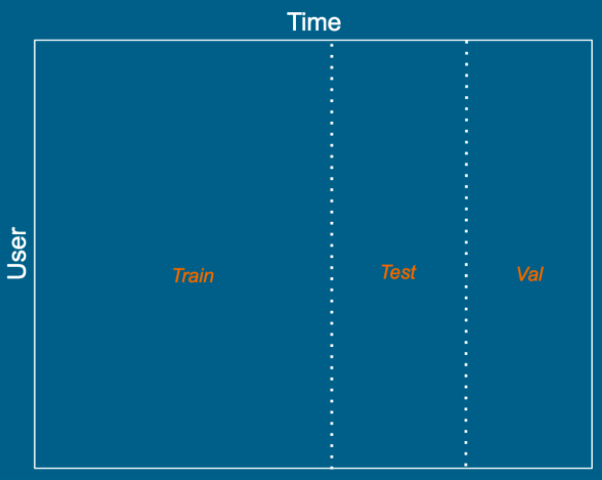
\includegraphics[width=2.5in]{stuff/rec3.png}\end{figure}}
\only<5-9>{\begin{figure}\centering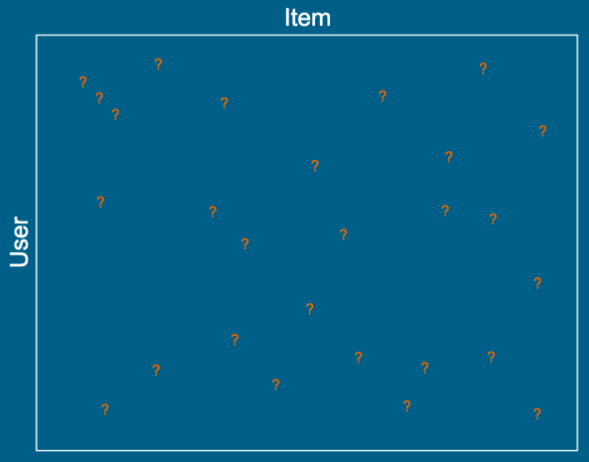
\includegraphics[width=2.5in]{stuff/rec5.png}\end{figure}}
\only<10->{\vspace{.85in}\hspace{6em}So many challenges...\\ \hspace{6em}A/B testing, anyone?\\
\vspace{1.1in}
}

\vspace{-1em}
\begin{itemize}
\item<2-> Leaving out items: \underline{doesn't works} (?)
\item<3-> Leaving out users: \underline{kind of works?} (?)
\item<4-> Scoring new users/itmes: \underline{a little late...} (?)
\begin{itemize}
\item \textcolor{Maroon}{User/Items Cold-Start} 
\end{itemize}
\end{itemize}

\end{column}
\hspace*{-2em}
\begin{column}{.5\textwidth}

\begin{itemize}
\item<5-> Scoring random user-items: \underline{train/test-ish} (?)
\item[]
\item<6-> Amazon really cares about your \textbf{buying}, not rating
\item<7->[] \emph{and what you want and your scores may be kinda different} 
\item<8-> Low scores aren't recommended so you shouldn't test on them
\item<9-> You don't have the items and scores that you should test on... \textcolor{gray}{that's the point: catch twenty-two...}
\end{itemize}

\end{column}
\end{columns}

}

\frame{
bleh
}


\end{document}





